
\begin{figure}[h]
    \centering

\tikzset{every picture/.style={line width=0.75pt}} %set default line width to 0.75pt        

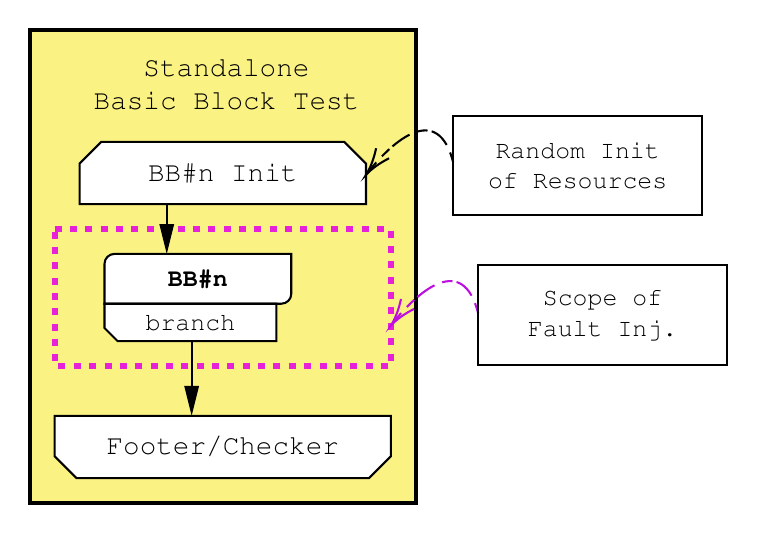
\begin{tikzpicture}[x=0.75pt,y=0.75pt,yscale=-1.2,xscale=1.2]
%uncomment if require: \path (0,385); %set diagram left start at 0, and has height of 385

%Shape: Rectangle [id:dp7916834050251116] 
\draw  [fill={rgb, 255:red, 248; green, 231; blue, 28 }  ,fill opacity=0.54 ][line width=1.5]  (375,140) -- (530,140) -- (530,330) -- (375,330) -- cycle ;
%Snip Same Side Corner Rect [id:dp7832878745055954] 
\draw  [fill={rgb, 255:red, 255; green, 255; blue, 255 }  ,fill opacity=1 ] (395,193.75) -- (403.75,185) -- (501.25,185) -- (510,193.75) -- (510,210) -- (510,210) -- (395,210) -- (395,210) -- cycle ;
%Shape: Rectangle [id:dp19676599731675015] 
\draw  [color={rgb, 255:red, 230; green, 33; blue, 215 }  ,draw opacity=1 ][dash pattern={on 2.53pt off 3.02pt}][line width=2.25]  (385,220) -- (520,220) -- (520,275) -- (385,275) -- cycle ;
%Rounded Diagonal Corner Rect [id:dp03911783521924184] 
\draw  [fill={rgb, 255:red, 255; green, 255; blue, 255 }  ,fill opacity=1 ] (405,234) .. controls (405,231.79) and (406.79,230) .. (409,230) -- (480,230) .. controls (480,230) and (480,230) .. (480,230) -- (480,246) .. controls (480,248.21) and (478.21,250) .. (476,250) -- (405,250) .. controls (405,250) and (405,250) .. (405,250) -- cycle ;
%Snip Single Corner Rect [id:dp49029702843535405] 
\draw  [fill={rgb, 255:red, 255; green, 255; blue, 255 }  ,fill opacity=1 ] (474.01,265) -- (410.25,265) -- (405,259.75) -- (405,250) -- (474.01,250) -- cycle ;
%Straight Lines [id:da003741804416257599] 
\draw    (440,265) -- (440,275) ;
%Straight Lines [id:da6294090718838072] 
\draw    (430,210) -- (430,228) ;
\draw [shift={(430,230)}, rotate = 270] [fill={rgb, 255:red, 0; green, 0; blue, 0 }  ][line width=0.08]  [draw opacity=0] (12,-3) -- (0,0) -- (12,3) -- cycle    ;
%Shape: Rectangle [id:dp024127327494653628] 
\draw   (545,174.5) -- (645,174.5) -- (645,214.5) -- (545,214.5) -- cycle ;
%Curve Lines [id:da39814587147130376] 
\draw  [dash pattern={on 3.75pt off 3pt on 7.5pt off 1.5pt}]  (545,193.25) .. controls (538.89,169.12) and (521.29,184.11) .. (511.08,196.87) ;
\draw [shift={(510,198.25)}, rotate = 307.57] [color={rgb, 255:red, 0; green, 0; blue, 0 }  ][line width=0.75]    (10.93,-3.29) .. controls (6.95,-1.4) and (3.31,-0.3) .. (0,0) .. controls (3.31,0.3) and (6.95,1.4) .. (10.93,3.29)   ;
%Curve Lines [id:da23423265564935447] 
\draw [color={rgb, 255:red, 189; green, 16; blue, 224 }  ,draw opacity=1 ] [dash pattern={on 3.75pt off 3pt on 7.5pt off 1.5pt}]  (555,253.75) .. controls (548.89,229.62) and (531.29,244.61) .. (521.08,257.37) ;
\draw [shift={(520,258.75)}, rotate = 307.57] [color={rgb, 255:red, 189; green, 16; blue, 224 }  ,draw opacity=1 ][line width=0.75]    (10.93,-3.29) .. controls (6.95,-1.4) and (3.31,-0.3) .. (0,0) .. controls (3.31,0.3) and (6.95,1.4) .. (10.93,3.29)   ;
%Shape: Rectangle [id:dp4792679092541773] 
\draw   (555,234.5) -- (655,234.5) -- (655,274.5) -- (555,274.5) -- cycle ;
%Snip Same Side Corner Rect [id:dp19614433052146063] 
\draw  [fill={rgb, 255:red, 255; green, 255; blue, 255 }  ,fill opacity=1 ] (520,311.25) -- (511.25,320) -- (393.75,320) -- (385,311.25) -- (385,295) -- (385,295) -- (520,295) -- (520,295) -- cycle ;
%Straight Lines [id:da35004371293914116] 
\draw    (440,275) -- (440,287.67) -- (440,293) ;
\draw [shift={(440,295)}, rotate = 270] [fill={rgb, 255:red, 0; green, 0; blue, 0 }  ][line width=0.08]  [draw opacity=0] (12,-3) -- (0,0) -- (12,3) -- cycle    ;

% Text Node
\draw (454,162) node   [align=left] {\begin{minipage}[lt]{120.64pt}\setlength\topsep{0pt}
\begin{center}
{\fontfamily{pcr}\selectfont Standalone }\\{\fontfamily{pcr}\selectfont Basic Block Test}
\end{center}

\end{minipage}};
% Text Node
\draw (452.5,197.5) node   [align=left] {{\fontfamily{pcr}\selectfont BB\#n Init}};
% Text Node
\draw (439.5,257.5) node  [font=\small] [align=left] {{\fontfamily{pcr}\selectfont branch}};
% Text Node
\draw (442.5,240) node  [font=\small] [align=left] {{\fontfamily{pcr}\selectfont \textbf{BB\#n}}};
% Text Node
\draw (595,194.5) node  [font=\small] [align=left] {\begin{minipage}[lt]{90.82pt}\setlength\topsep{0pt}
\begin{center}
{\fontfamily{pcr}\selectfont Random Init }\\{\fontfamily{pcr}\selectfont of Resources}
\end{center}

\end{minipage}};
% Text Node
\draw (605,254.5) node  [font=\small] [align=left] {\begin{minipage}[lt]{85.8pt}\setlength\topsep{0pt}
\begin{center}
{\fontfamily{pcr}\selectfont Scope of}\\{\fontfamily{pcr}\selectfont Fault Inj.}
\end{center}

\end{minipage}};
% Text Node
\draw (452.5,307.5) node   [align=left] {{\fontfamily{pcr}\selectfont Footer/Checker}};


\end{tikzpicture}
    \caption{Block Diagram of the Entire SW Product}
    \label{complete_sw}
\end{figure}
